\mcmSection{模型的建立与求解}

\mcmSubsection{问题1:通过三角函数求出多波束探测的覆盖宽度}

根据题意,可以抽象出如下的几何问题。

已知$\vartriangle PAB$是以$PA$、$PB$为腰的等腰三角形,其中,点$C$是$BP$上任意一点, PM是AB的垂线,且$\angle APB = \theta$, $\angle CAB = \alpha$, $PM = D$(如图\ref{fig:理想情况下的覆盖区域几何图}),求出$AC$在$AB$上的投影。

\begin{figure}[h]
    \centering
    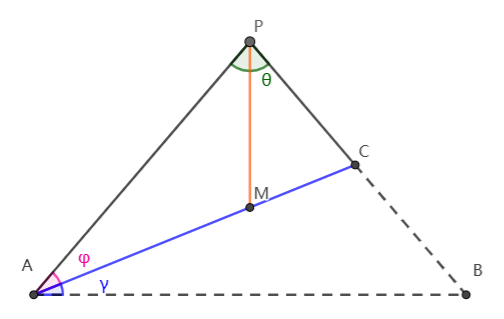
\includegraphics[scale=0.4]{res/img/理想情况下的覆盖区域几何图.png}
    \caption{理想情况下的覆盖区域几何图}
    \label{fig:理想情况下的覆盖区域几何图}
\end{figure}

由题意可设$AM=x_1$,$MC=x_2$,$\angle PAM = \frac{\pi - \theta}{2} - \alpha = \varphi $.

对于$\vartriangle PAM$,根据正弦定理,存在方程:

\begin{equation}
    \frac{\sin\angle APM}{AM} = \frac{\sin\angle PAM}{PM}
\end{equation}

对于$\vartriangle PCM$,根据正弦定理,存在方程:

\begin{equation}
    \frac{\sin\angle CPM}{CM} = \frac{\sin\angle PCM}{PM}
\end{equation}

综上所述,将对应的值带入方程,可得下列方程组:

\begin{equation}
    \begin{cases}
        \varphi = \frac{\pi - \theta}{2} - \alpha \\
        \frac{\sin \frac{\theta}{2}}{x_1} = \frac{\sin\varphi}{D} \\
        \frac{\sin \frac{\theta}{2}}{x_2} = \frac{\sin(\pi-\theta-\varphi)}{D}
    \end{cases}
\end{equation}

解得

\begin{equation}
    AC = x_1 + x_2 
       = \frac{\sin\frac{\theta}{2}}{\sin\varphi}D + \frac{\sin\frac{\theta}{2}}{\sin(\pi - \theta - \varphi)}D
\end{equation}

故

\begin{equation}
    Proj AC = \left(\frac{\sin\frac{\theta}{2}}{\sin\varphi}D + \frac{\sin\frac{\theta}{2}}{\sin(\pi - \theta - \varphi)}D\right) \cdot \cos \alpha
    \label{equ:理想情况下的区域覆盖公式}
\end{equation}

根据公式\ref{equ:理想情况下的区域覆盖公式},根据实际参数,编程(后面指出具体是哪个代码)后可得出下列结果:

% Please add the following required packages to your document preamble:
% \usepackage{booktabs}
\begin{table}[h]
    \centering
    \caption{\textbf{问题1的计算结果}}
    \begin{tabular}{@{}ccllllllll@{}}
    \toprule
    测线距中心点处的距离/$m$  & $-800$ & $-600$ & $-400$ & $-200$ & $0$ & $200$ & $400$ & $600$ & $800$ \\ \midrule
    海水深度/$m$        &      &      &      &      & 70  &     &     &     &     \\
    覆盖宽度/$m$        &      &      &      &      &   &     &     &     &     \\
    与前一条测线的重叠率/$\%$ &   -  &      &      &      &   &     &     &     &     \\ \bottomrule
    \end{tabular}
\end{table}


\mcmSubsection{问题二:一般情况下,覆盖率求解}

根据题意,可以抽象出如下的几何问题:

有两个直三棱柱如图\ref{fig:一般情况下的覆盖区域几何图}所示摆放,三棱柱$BEC-AFD$的侧边与三棱柱$DHC-FGE$的侧边相重合(这里用词是否准确?),其中,$AF$垂直于$FE$,$FG$垂直于$GE$,$\angle AFG=\beta$,$\angle CBE=\alpha$。设平面$ABCD$与平面$HCEG$的交线为$l_s$,求$l_s$与$ABEF$平面的夹角。

\begin{figure}[h]
    \centering
    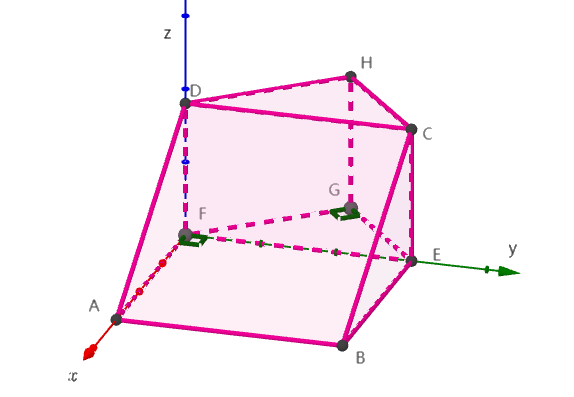
\includegraphics[scale=0.4]{res/img/一般情况下的覆盖区域几何图.png}
    \caption{一般情况下的覆盖区域几何图}
    \label{fig:一般情况下的覆盖区域几何图}
\end{figure}

分别设平面ABCD与平面HCEG的法向量为$\tau_\text{坡}$和$\tau_\text{测}$,$l_s$的方向向量为$v_s$.

根据平面法向量的性质,存在方程组:

\begin{equation}
    \begin{cases}
        \tau_\text{坡} \cdot v_s = 0 \\
        \tau_\text{测} \cdot v_s = 0
    \end{cases}
\end{equation}

又因为$\angle AFG=\beta$,$\angle CBE=\alpha$,可得:

\begin{equation}
    \begin{cases}
        \tau_\text{坡} = (\sin\alpha, 0, \cos\alpha) \\
        \tau_\text{测} = (-\sin(\beta-\frac{\pi}{2}), \cos(\beta-\frac{\pi}{2}), 0)
    \end{cases}
\end{equation}

故有方程组:

\begin{equation}
    \begin{cases}
        x\sin\alpha + z\cos\alpha = 0 \\
        -x\sin(\beta-\frac{\pi}{2}) + y \cos(\beta-\frac{\pi}{2}) = 0
    \end{cases}
\end{equation}

综上所述,可得

\begin{equation}
    v_s 
    = (i, j, k)
    = \left( 
            \cot \alpha, 
            \frac{\cot\alpha \sin\left(\beta - \frac{\pi}{2}\right)}{\cos\left(\beta-\frac{\pi}{2}\right)},
            -1
            \right)
\end{equation}

所以,$l_s$与平面$ABEF$的夹角为

\begin{equation}
    <l_s, ABEF> = \arctan\frac{k}{\sqrt{i^2+j^2}}
\end{equation}

\mcmSection{模型的评价与改进}